% day3_seg1_navproblem/strapdown.tex
\begin{frame}
Strapdown Navigation:  Strapdown vs. Gimbaled
\begin{itemize}
  \item Gimbaled INS:
  \begin{itemize}
	\item Gyro stabilized platform
	\item Gimbal assembly and torque motors
	\item Resolvers, slip rings, bearings, etc. to control  platform
	\item Goal: Maintain stable, locally level or inertial reference frame
  \end{itemize}
\end{itemize} 
\end{frame}


\begin{frame}
Strapdown Navigation: Strapdown vs. Gimbaled
\begin{itemize}
  \item Gimbaled INS Issues
  \begin{itemize}
	\item Reliability and Cost: Lots of moving parts!
	\item Body rate and acceleration information not directly available
	\item Rate signals are generally noisy and have low bandwidth
  \end{itemize}
\end{itemize} 
\end{frame}


\begin{frame}
Strapdown Navigation: Strapdown vs. Gimbaled
\begin{itemize}
  \item Strapdown INS:
  \begin{itemize}
	\item Inertial instruments strapped to body frame
	\item Requires local level accelerations to be computed using direction cosine matrix $\dcm{B}{L}$
	\item $\dcm{B}{L}$ derived from gyro-sensed body rates
    \item Strapdown systems can be implemented with either rate gyros or attitude gyros 
  \end{itemize} 
\end{itemize} 
\end{frame}

\begin{frame}
Strapdown Navigation: Strapdown vs. Gimbaled
\begin{itemize}
  \item Strapdown INS Advantages
  \begin{itemize}
	\item Immediate detection of body rates and accelerations
	\item Fewer moving parts
	\item Potential redundancy advantages
  \end{itemize} 
  \item Gimbaled systems are nearly obsolete
\end{itemize} 
\end{frame}

\begin{frame}
%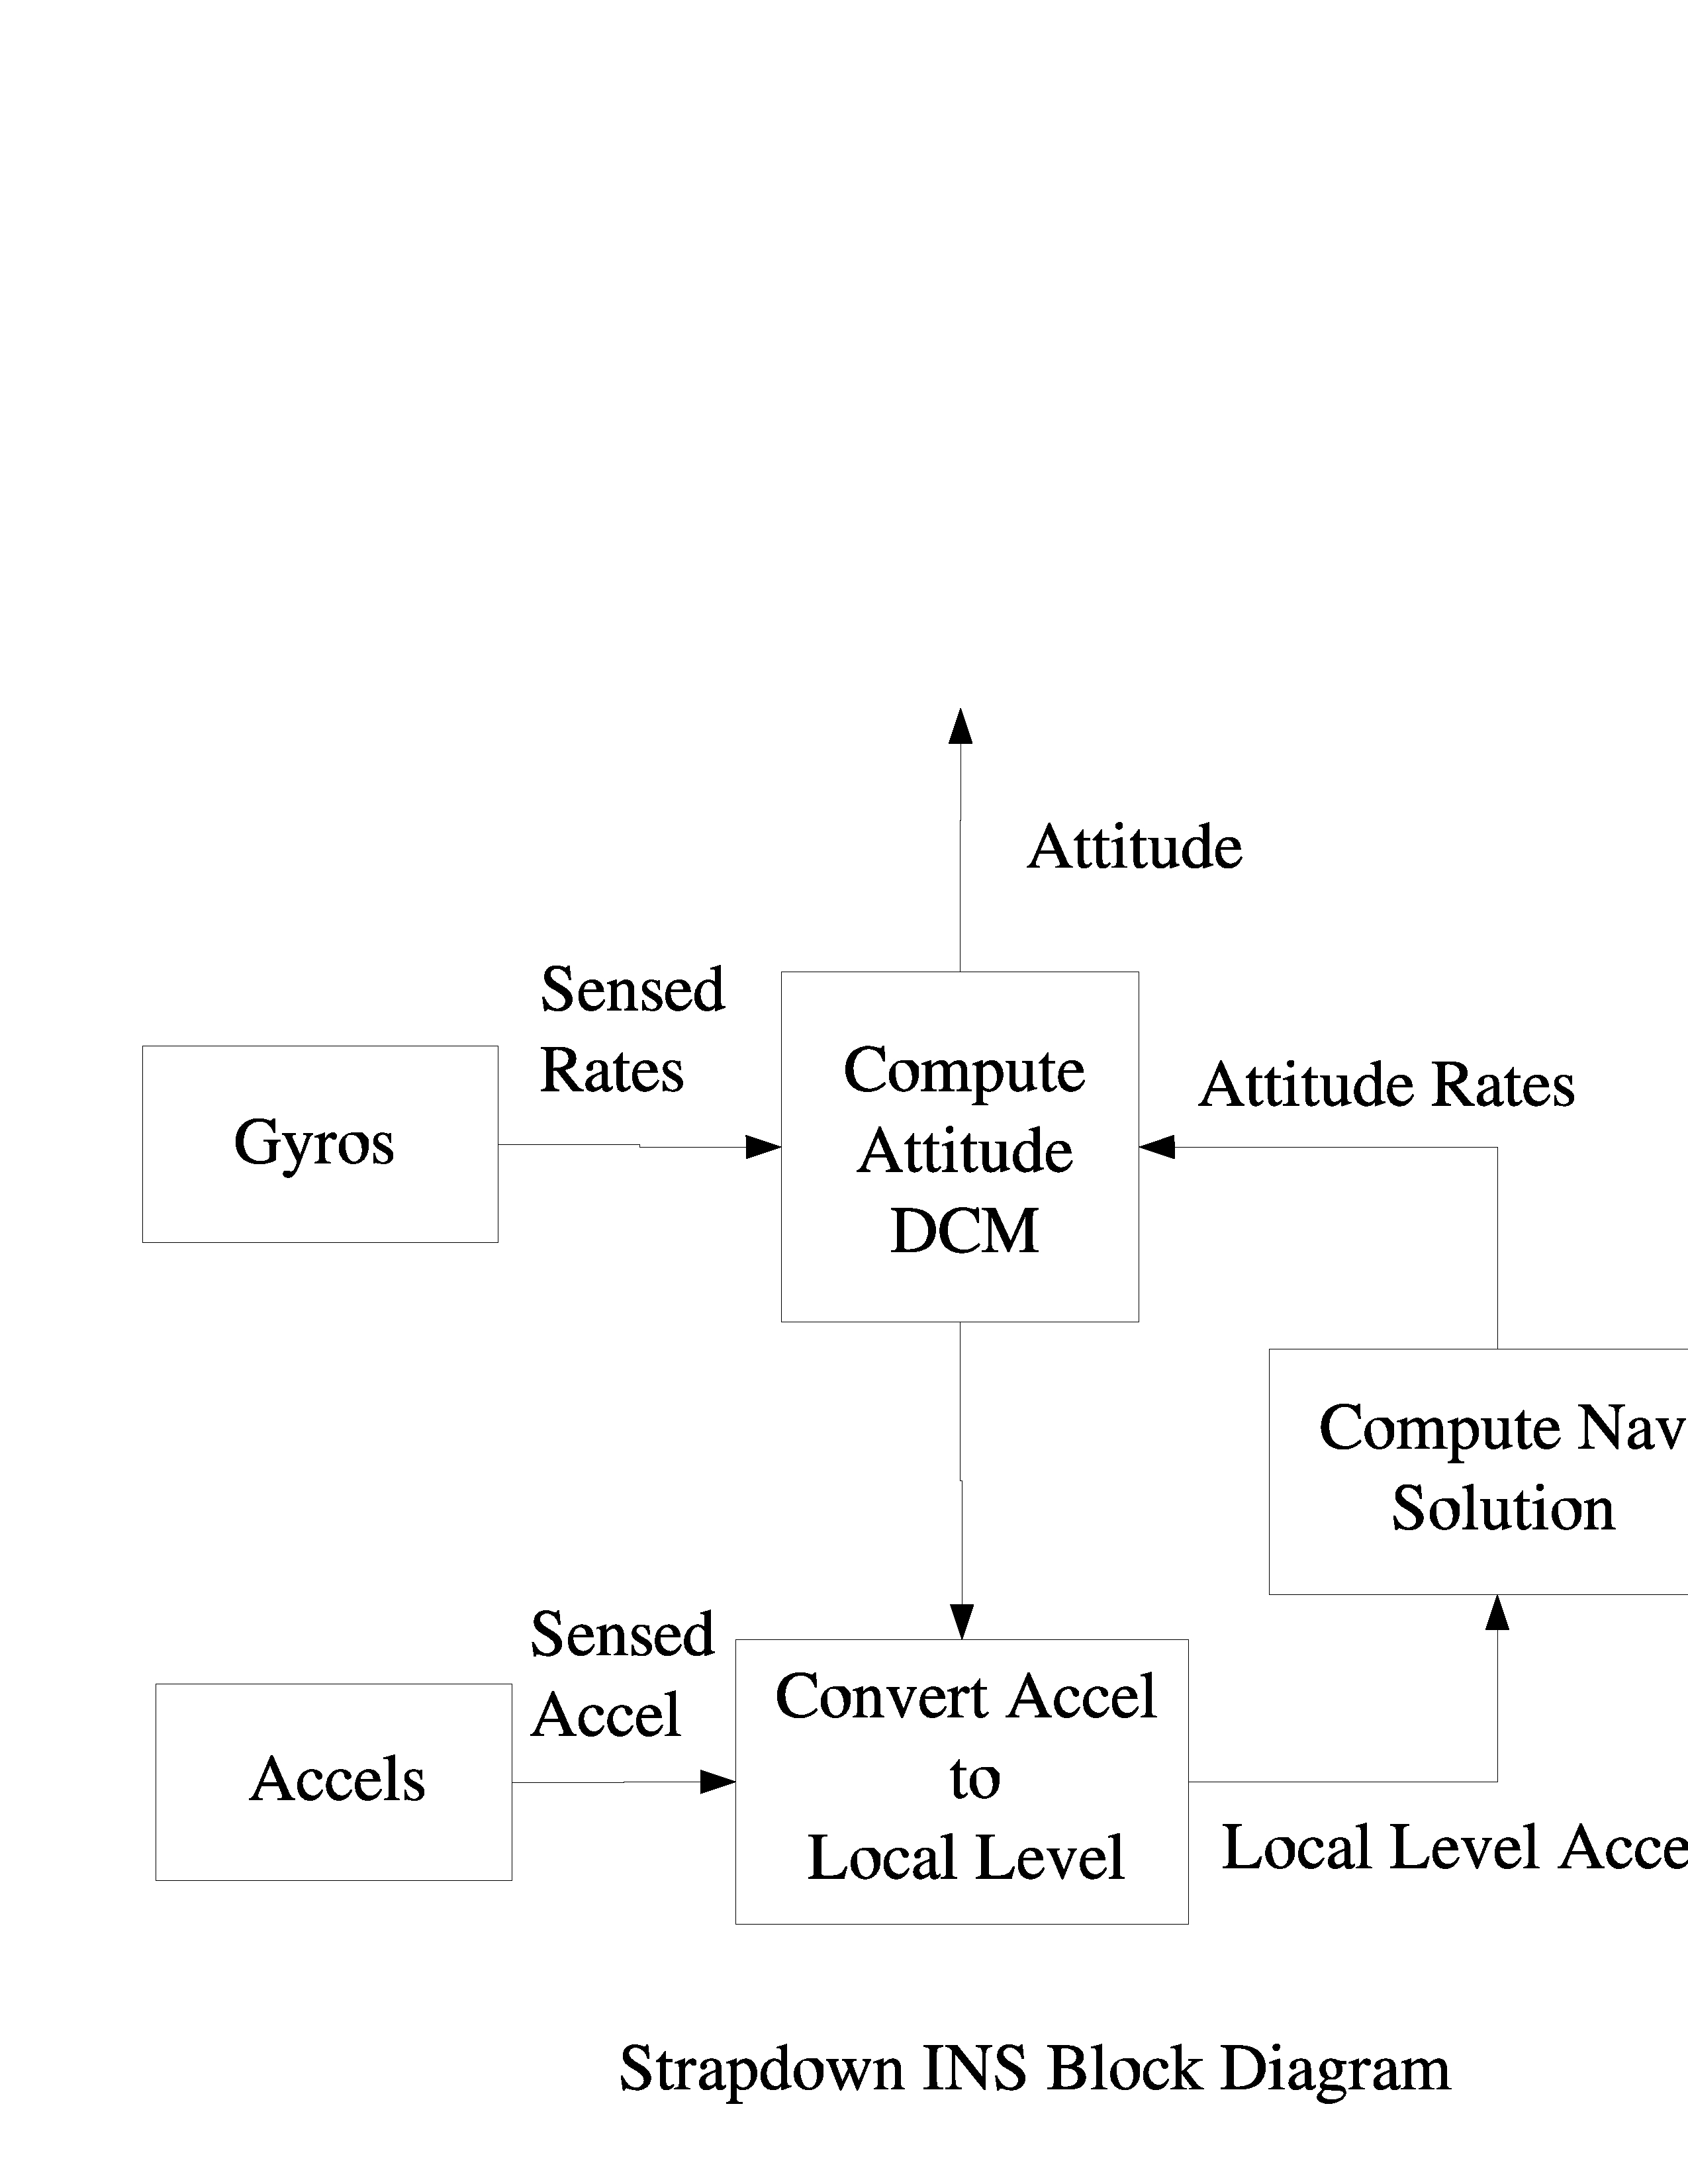
\includegraphics[width=\textwidth]{graphics/strapdown_block.jpg}
\end{frame}

\begin{frame}
Basic Strapdown Navigation Equations
 \begin{itemize}
 \item Need to compute attitude, velocity, and position
 \item I.e., need to compute $\dcm{B}{L}$ and $\dcm{L}{E}$
 \item These DCMs are dynamic quantities
 \item $\dcm{B}{L}$ determines attitude and can be rapidly varying
 \item $\dcm{L}{E}$ determines position and is slowly varying (relative to attitude dynamics)
\end{itemize}
\end{frame}

\begin{frame}
Rotating Coordinate Frames
\begin{itemize}
\item We first need to understand how an arbitrary vector and its time
derivatives in one coordinate frame are expressed in another frame
that is rotating with respect to the first.  
\item Let $A$ and $B$
denote two coordinate frames and assume that $B$ is rotating with
respect to $A$.  
\item We use the notation $\rotvec{A}{B}^A$ to express
the direction and magnitude of the rotation vector as seen in the $A$ frame.
\end{itemize}
\end{frame}
\begin{frame}
Rotating Coordinate Frames
\begin{itemize}
\item Every rotation vector can also be expressed as a skew symmetric
matrix.  
\item If $\omega$ is a rotation vector (without mentioning the
frames involved), then
\[\Omega = \skewsymmat{\omega}{1}{2}{3}.\]
\end{itemize}
\end{frame}
\begin{frame}
Rotating Coordinate Frames
\begin{itemize}
\item Since multiplication of a vector by the skew symmetric matrix
equivalent is the same thing as left multiplying the cross product
of the original vector, we can write:
\[\Omega v = \omega \times v\]
\item Therefore the notation $\xop{\omega}=\Omega$ is
common\footnote{One must be careful in making this identification
since left matrix multiplication is associative while left cross
product multiplication is not.}
\end{itemize}
\end{frame}

\begin{frame}
Rotating Coordinate Frames
\begin{itemize}
\item Let $v$ be an arbitrary vector in 3-space. 
\item Let
$\set{e_A^1,e_A^2,e_A^3}$ be orthonormal basis vectors in the $A$
frame 
\item Let $\set{e_B^1,e_B^2,e_B^3}$ be orthonormal basis
vectors in the $B$ frame\footnote{We reverse the roles of superscripts
and subscripts for basis vectors so that we may employ the
Einstein summation convention on occasion.}.  
\end{itemize}
\end{frame}

\begin{frame}
Rotating Coordinate Frames
\begin{itemize}
\item Thus, we can write
$v$ as $\sum_{i=1}^3 v_i^A e_A^i$ and also $\sum_{i=1}^3 v_i^B
e_B^i$. 
\item This is one and the same vector expressed in two different
coordinate frames\footnote{A vector is a linear combination of
basis vectors and not necessarily an ordered triple of real numbers.}.
\end{itemize}
\end{frame}
\begin{frame}
Rotating Coordinate Frames
\begin{itemize}
\item Note that, with respect to an arbitrary inertial
reference frame, we have for the time derivative:
\begin{align*}
  v &= \sum_{i=1}^3 v_i^A e_A^i = \sum_{i=1}^3 v_i^B e_B^i\\
    &\Rightarrow  \dot{v} = \dfrac{d}{dt}\left[ \sum_{i=1}^3 v_i^A e_A^i \right] = \dfrac{d}{dt}\left[\sum_{i=1}^3 v_i^B e_B^i
    \right]\\
    &\Rightarrow \sum_{i=1}^3 \left( \dot{v}_i^A e_A^i+ v_i^A
    \dot{e}_A^i\right)
    = \sum_{i=1}^3 \left(\dot{v}_i^B e_B^i+ v_i^B \dot{e}_B^i\right)\\
\end{align*}
\end{itemize}
\end{frame}
\begin{frame}
Rotating Coordinate Frames
\begin{itemize}
\item In the special case
that their respective coordinate frames are not rotating relative
to one another, each $\dot{e}_A^i = 0 = \dot{e}_B^i$.   
\item Nevertheless, regardless of rotation, we must always have:
\begin{equation}\label{scalarinveq}
  \scalarinveq.
\end{equation}
(Note that, in general, $\dot{v}_i^A\neq\dot{v}_i^B$.)
\end{itemize}
\end{frame}
\begin{frame}
Rotating Coordinate Frames
\begin{itemize}
\item Let frame $B$ rotate with respect to frame $A$ at a constant
rotational rate $\rotvec{A}{B}^A$ as expressed in $A$ frame coordinates.  
\item Since $B$ is not rotating with respect to itself, let us agree to label the quantity in Eq. \eqref{scalarinveq} as
$\dot{v}^B$. 
\item We'll assume that $A$ is an inertial frame and thus $\dot{v}=\dot{v}^A$.
\end{itemize}
\end{frame}
\begin{frame}
Rotating Coordinate Frames
\begin{itemize}
\item When viewed from the $A$ frame, however, it is not true that each
of the $\dot{e_i}^B$ is zero, since these unit vectors are slaved
to the $B$ frame and $B$ is rotating with respect to $A$ at rate
$\rotvec{A}{B}^A$.  
\item Therefore, we have:
\begin{equation}\label{aderiv}
\begin{split}
\dot{v}^A&=\sum_{i=1}^3 \dot{v}_i^A e_A^i + \sum_{i=1}^3 v_i^B
\dot{e}_B^i\\
         &=\sum_{i=1}^3 \dot{v}_i^B e_B^i + \sum_{i=1}^3 v_i^B
\dot{e}_B^i \text{\;\;\;\;(by Eq. \eqref{scalarinveq})}\\
         &=\dot{v}^B +\sum_{i=1}^3 v_i^B\dot{e}_B^i.
\end{split}
\end{equation}
\end{itemize}
\end{frame}

\begin{frame}
Rotating Coordinate Frames
\begin{itemize}
\item The last sum on the right side of Eq. \eqref{aderiv} can be
rewritten as the cross product $\rotvec{A}{B}^A\times v$, because
$\dot{e}_B^i=\rotvec{A}{B}^A\times e_B^i$, and
\begin{align*}
   \sum_{i=1}^3 v_i^B\dot{e}_B^i &= \sum_{i=1}^3 v_i^B\rotvec{A}{B}^A\times e_B^i \\
  &=\rotvec{A}{B}^A\times \sum_{i=1}^3 v_i^B e_B^i \\
  &=\rotvec{A}{B}^A\times v.
\end{align*}
\end{itemize}
\end{frame}
\begin{frame}
Rotating Coordinate Frames
\begin{itemize}
\item We thus arrive at the all-important Coriolis Equation which is
used often in navigation analysis:
\begin{equation}\label{corioliseq}
  \corioliseq.
\end{equation}
\end{itemize}
\end{frame}
\begin{frame}

Alternatively, we can express Eq. \eqref{corioliseq} in
skew-symmetric matrix form using
$\rotmat{A}{B}=\xop{\rotvec{A}{B}}$:
\begin{equation}\label{coriolismateq}
  \coriolismateq.
\end{equation}

Note that we must use superscripts on both $\rotmat{A}{B}$ and $v$
as soon as we make a commitment to a particular coordinate frame
representation.\footnote{Since matrices are defined in terms of
their action on basis vectors, it is appropriate to specify the
coordinate system.  On the other hand, if $\rotmat{A}{B}$ is taken
to be a linear transformation, then superscripts are not
necessary.}.

\end{frame}


\begin{frame}
Strapdown Navigation Equations
 \begin{itemize}
 \item Three differential equations
 \begin{itemize}
   \item Equation for body to local level transformation $\dcm{B}{L}$
   \item Equation for velocity (uses $\dcm{B}{L}$)
   \item Equation for local level to earth for position DCM $\dcm{L}{E}$
 \end{itemize}
\end{itemize}
\end{frame}
\begin{frame}
Strapdown Navigation Equations
 \begin{itemize}
 \item Two Algebraic Equations
 \begin{itemize}
   \item Equation for converting velocity to transport rate (to be explained)
   \item Equation for converting earth rate to local level
   coordinates
 \end{itemize}
\end{itemize}
\end{frame}
\begin{frame}
Strapdown Navigation Equations\\
The Three Differential Equations\\
\begin{equation}\label{cbleq}
  \cbleq
\end{equation}
\begin{equation}\label{strapveleq}
  \strapveleq
\end{equation}
\begin{equation}\label{cleeq}
  \cleeq
\end{equation}
\end{frame}
\begin{frame}
Strapdown Navigation Equations\\
The Two Algebraic Equations\\
\begin{equation}\label{trateeq}
  \trateeq \text{ (wander azimuth $\rho_z=0$)}
\end{equation}
\begin{equation}\label{erateeq}
  \erateeq
\end{equation}
\end{frame}
\begin{frame}
Strapdown Navigation Equations\\
The $\dcm{B}{L}$ Equation \eqref{cbleq}
\[\cbleq\]
\begin{itemize}
\item All the $\Omega$ matrices represent rotation vector cross products in skew-symmetric matrix format
\begin{itemize}
 \item $\rotmat{I}{B}^B$ is rotational rate of aircraft in body
coordinates
\item $\rotmat{I}{E}^L$ is earth rate in local level coordinates
\item $\rotmat{E}{L}^L$ is transport rate in local level
coordinates
\end{itemize}
\end{itemize}
\end{frame}
\begin{frame}
Strapdown Navigation Equations: Detour into Cross Product Matrices\\
\begin{itemize}
\item The cross product of $\omega=\colvecthree{\omega}{}$ with any other vector $v$ is the same as multiplying $v$ on the left by
$\Omega = \skewsymmat{\omega}{1}{2}{3}$
\item $\omega \times v=\Omega v$
\end{itemize}
\end{frame}
\begin{frame}
Strapdown Navigation Equations\\
The $\dcm{B}{L}$ Equation \eqref{cbleq}
\[\cbleq\]
\begin{itemize}
\item Transport rate is the rotational rate of the aircraft due to
motion over the surface of the earth.  Is a function of velocity.
\item $\rotmat{I}{B}^B$ is total inertial angular rate sensed by gyros and includes effects of
transport and earth rates.
\item Hence transport and earth rate effects have to be subtracted
off.
\end{itemize}
\end{frame}
\begin{frame}
Strapdown Navigation Equations\\
The Strapdown Velocity Equation \eqref{strapveleq}
\[\strapveleq\]
 \begin{itemize}
 \item Sometimes referred to as the velocity rate equation
 \item $\specforce^B$ is specific force sensed by accelerometers in
 body coordinates (because the accels are strapped to the body --
 hence the term strapdown)
\end{itemize}
\end{frame}
\begin{frame}
%\includegraphics[width=10in,height=6.5in]{strapnav_block.jpg}
\end{frame}
\begin{frame}
Strapdown Navigation Equations\\
The Transport Rate Equation \eqref{cleeq}
\[\cleeq\]
\begin{itemize}
  \item Connected to velocity rate equation by the first algebraic equation \eqref{trateeq}:
\[\trateeq\]
  \item Eq. \eqref{cleeq} Sometimes referred to as position rate equation, because $\dcm{L}{E}$ directly implies the vehicle position
\end{itemize} 
\end{frame}

\begin{frame}
Strapdown Navigation Equations\\
Position Rate / Transport Rate Equations (Geographic)
\begin{itemize}
  \item North transport rate:
\begin{equation}\label{trateneq}
\trateneq
\end{equation} 
  \item East transport rate:
\begin{equation}\label{trateeeq}
\trateeeq
\end{equation} 
where $e$ is ellipticity (approx. $\dfrac{1}{298}$) and $R_e$ is mean equatorial earth radius
\end{itemize} 
\end{frame}

\begin{frame}
Strapdown Navigation Equations\\
Position Rate / Transport Rate Equations (Geographic)
\begin{itemize}
  \item Latitude Rate:
\begin{equation}\label{latrate}
\latrateeq
\end{equation}  
  \item Longitude Rate:
\begin{equation}\label{lonrate}
\lonrateeq
\end{equation}  
\end{itemize} 
\end{frame}

\begin{frame}
Strapdown Navigation Equations\\
\begin{itemize}
  \item Geographic (north-slaved) mechanization has singularities at poles
  \item Two other approaches to local level coordinates:
  \begin{itemize}
	\item Free azimuth: vertical component of transport rate $\rho_z$= additive inverse of vertical component of earth rate
	\item Wander Azimuth:  vertical component of transport rate $\rho_z$ = 0
  \end{itemize}
\end{itemize} 
\end{frame}

\begin{frame}
Strapdown Navigation Equations\\
Position Rate / Transport Rate Equations (Wander and Free Azimuth)
\begin{itemize}
  \item X Transport Rate:
\begin{align}\label{xtrateeq}
\xtrateeq
\end{align}  
  \item Y Transport Rate:
\begin{align}\label{ytrateeq}
\ytrateeq
\end{align}  
\end{itemize} 
\end{frame}

\begin{frame}
Strapdown Navigation Equations\\
Position Rate / Transport Rate Equations (Wander and Free Azimuth)
\begin{itemize}
  \item Azimuth Rate:
\[
\rho_z= 
\begin{cases} 
-\erate d_{23}, &\text{if free azimuth;}\\ 
0,  &\text{if wander azimuth} 
\end{cases}
\]
  \item In equations above, the matrix $\left[d_{ij}\right]$ is the direction cosine matrix $\dcm{L}{E}$ from local level (L) frame to earth centered earth fixed (E) frame.
\end{itemize} 
\end{frame}
